\documentclass{article}
\usepackage{geometry}                % See geometry.pdf to learn the layout options. There are lots.
\geometry{a4paper}                   % ... or a4paper or a5paper or ... 
%\geometry{landscape}                % Activate for for rotated page geometry
%\usepackage[parfill]{parskip}    % Activate to begin paragraphs with an empty line rather than an indent
\usepackage{graphicx}
\usepackage{amssymb}
\usepackage{amsthm}
\usepackage{amsmath}
\usepackage{mathrsfs}
\usepackage[french]{babel}
\usepackage{color}
\usepackage{listings}
\definecolor{javared}{rgb}{0.6,0,0} % for strings
\definecolor{javagreen}{rgb}{0.25,0.5,0.35} % comments
\definecolor{javapurple}{rgb}{0.5,0,0.35} % keywords
\definecolor{javadocblue}{rgb}{0.25,0.35,0.75} % javadoc

\lstset{language=Java,
basicstyle=\ttfamily,
keywordstyle=\color{javapurple}\bfseries,
stringstyle=\color{javared},
commentstyle=\color{javagreen},
morecomment=[s][\color{javadocblue}]{/**}{*/},
stepnumber=2,
numbersep=10pt,
tabsize=4,
showspaces=false,
showstringspaces=false}
\usepackage[applemac]{inputenc}
\newtheorem{theorem}{Th�or�me}
\newtheorem*{definition}{D�finition}
\newtheorem*{exercice}{Exercice}
\hyphenpenalty=10000

\title{Secure Airport Tower\\First Development Journal}
\author{frederic.jacobs@epfl.ch\\ hantao.zhao@epfl.ch}
\begin{document}
\maketitle 
\section{Setting up}
During the set up phase, we chose Git over SVN. There are many reasons that explain this decision but we'll highlight here only a few. We really fancy the social features of GitHub for collaboration. GitHub Issues makes it easier to report bugs and to fix them. Git is also way simpler to set up than SVN. The branching of Git makes it way easier to work on different branches and then merge them with the master at a further stage. We set it up as a private repository according to the requirements of this course.
\section{Project's Architecture}
Our program is structured into different packages.

\begin{figure}[h]
  \centering
  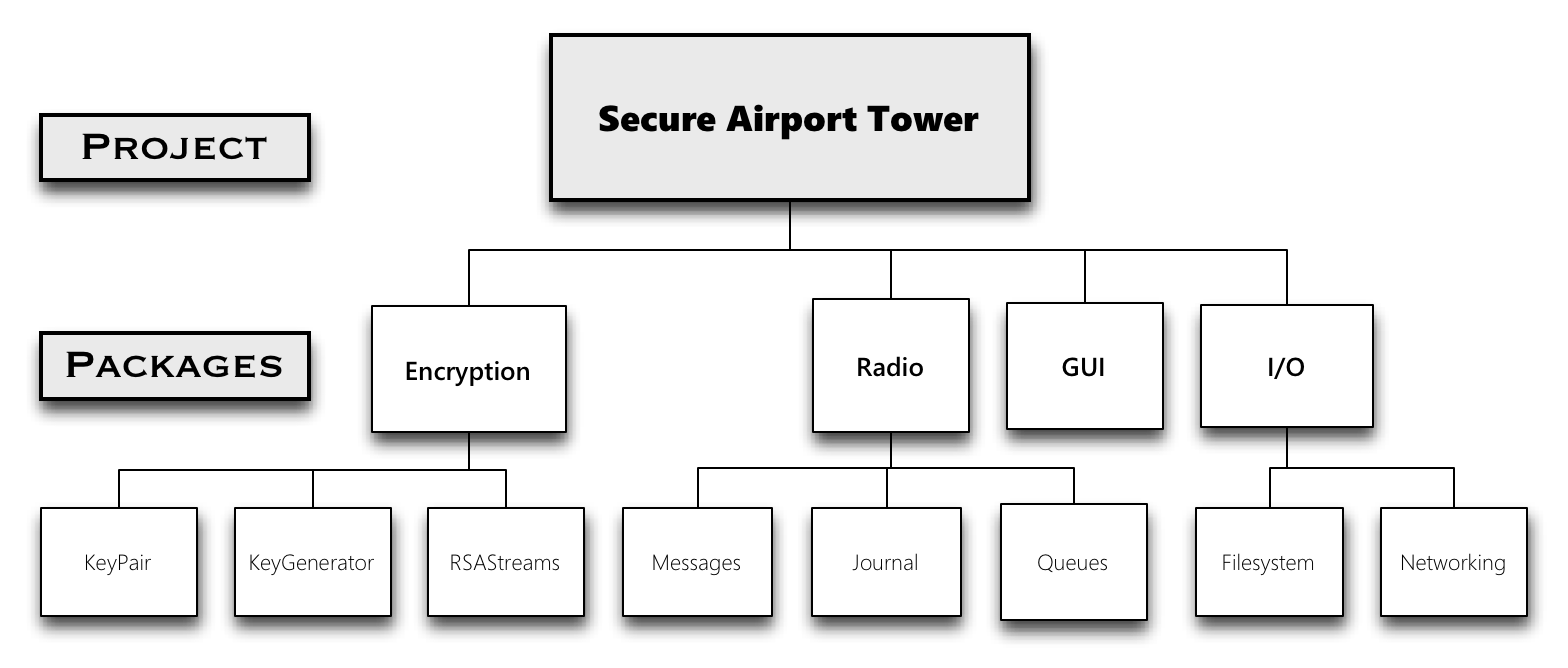
\includegraphics[width=\textwidth]{Architecture.png}
  \caption{The current architecture of our software. It is subject to change in later iterations for consistency.} 
\end{figure}

\subsection{Encryption}
This package contains two main classes namely \emph{KeyPair}, which can store both public and private keys, and \emph{KeyGenerator}, which can generate both public and private keys with a given length during the initialization of the program. In addition of these two classes we coded a \emph{RSAInputStream} and  \emph{RSAOutputStream} which can handle encryption and decryption of incoming and outgoing streams.
\subsection{GUI}
The Graphical User Interface hasn't been coded yet but the package is already there, waiting to be implemented. 
\subsection{I/O}
At this current stage of development we haven't coded the network support yet. Thus, we built a custom class to write the messages in the filesystem instead of sending them straight to the network.
\subsection{Radio}
The Radio handles all messaging by sorting them into priority queues. The radio package also holds all of the Message classes which defines what the messages contains. We also provide support for data messages (using the I/O package to get some special hash treatment).

\section{Q\&A}
In ITP-02, we were asked two questions. 
\begin{enumerate}
\item Is it a good idea to use a superclass to define Messages ?
\item Why is it an abstract class ?
\end{enumerate}
In a object-oriented universe like Java, we like to model things hierarchically. We want all possible types of messages to have a behavior or to have some instance variables therefore defining a super-class Messages makes a lot of sense. We were asked to have these instance variables in each Message Type so we implemented these in our super-class.

\begin{lstlisting}
byte[] planeID;  //The unique identifier of the plane
int length; //Length of the message
int priority; //Priority in PriorityQueue
int posx; //Positioning data 
int posy;
MessageType type; //Type of Message
\end{lstlisting}

The reason why we want this to be an abstract class is really straightforward. We defined a Message super-class because we expect messages to behave a given way but we also want these messages to have a type. All messages will inherit these attributes from the super-class but the super-class won't be instantiable to assure we call the right constructor when creating a message with a certain type. The keyword \emph{abstract} does exactly this. 

\end{document}


Pri�re d�ajouter une r�ponse synth�tique � ces questions sur votre journal :
1. Avoir une super classe dans ce cas. Est-??ce une bonne id�e ?
2. Pourquoi serait-??elle une classe abstraite ?

